\label{axon1dcommander}

\begin{figure}[h]
\begin{center}
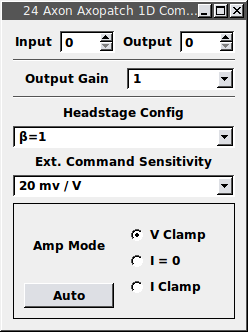
\includegraphics[width=2in]{axon1d.png}
\caption[axon1d]{The Axon Axopatch 1D Commander.}
\end{center}
\end{figure}

The settings of the module must match the settings of the Output Gain, Headstage Config, Ext. Command Sensitivity, and mode set by the amplifier's switches. The module is able to accept the amplifier's Gain Telegraph, allowing it to sense changes to the gain knob of the amplifier. It is also able to sense the mode of the amplifier through its Mode Telegraph. These are both located on the back of the amplifier.

input(0) - "Mode Telegraph" : The analog voltage signal from the amplifier's mode telegraph, allowing the module to determine the mode of the amplifier when the auto button is toggled

input(1) - "Gain Telegraph" : The analog voltage signal from the amplifier's gain telegraph, allowing the module to determine the gain set when the auto button is toggled.